\chapter{El algoritmo}

El cálculo de la dimensión fractal de una estructura de datos proporciona información relevante sobre la propia estructura, ya que el análisis fractal analiza su estructura geométrica a múltiples niveles.\\

El método utilizado en este proyecto se llama Box counting. Su funcionamiento reside en la subdivisión de la estructura de datos en cajas, con el objetivo de poder analizar la estructura en una escala más pequeña. El nombre de Box counting viene dado ya que el algoritmo, en esencia, lo que hace es contar la cantidad de cajas (de distintos tamaños) que hay en la estructura. Por esto mismo, antes decíamos que el análisis fractal analiza la estructura a múltiples niveles, porque el algoritmo empieza contando cajas de la menor dimensión posible (1) y acaba por contar las cajas de mayor tamaño posible (el de la estructura de datos).\\

Cuando aplicamos el algoritmo Box counting, nos interesa el cálculo de dos medidas:


\begin{itemize}
    \item \textbf{N}: Representa el número de cajas \textit{válidas} que hay presentes en la estructura.
    \item \textbf{r}: Representa el tamaño de las cajas. 
\end{itemize}
 
Como ya se ha comentado antes, el algoritmo realiza un análisis multinivel de la estructura, es decir que no solo obtenemos un valor de N y otro de r, si no que para cada valor de r (es decir, para cada tamaño de la caja) obtenemos un valor de N (una cantidad de cajas de tamaño r). El cálculo de la dimensión fractal (D) viene dado por la siguiente expresión \ref{formula}.

En las Figuras \ref{fig:basico1} y \ref{fig:basico2} , se aprecia el análisis multinivel del que hablamos. En función del tamaño de la caja el número de cajas válidas cambia.

\begin{equation}
    \label{formula}
    D = \frac{log(N)}{log(r)}
\end{equation}

\begin{figure}[H]
    \centering
    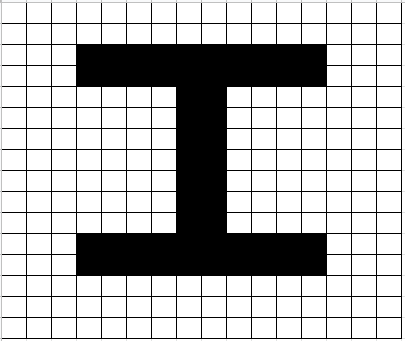
\includegraphics[width=.24\textwidth]{img/basico1.png}
    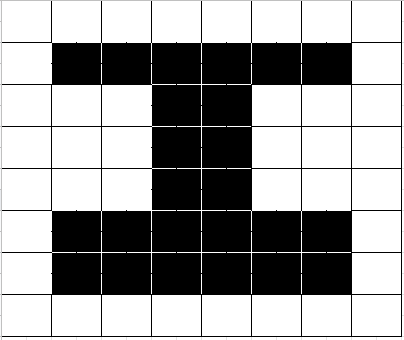
\includegraphics[width=.24\textwidth]{img/basico2.png}
    \caption{Simplificación algoritmo con r = 1 (Izquierda) y r = 2 (Derecha)}
    \label{fig:basico1}
\end{figure}

\begin{figure}[H]
    \centering
    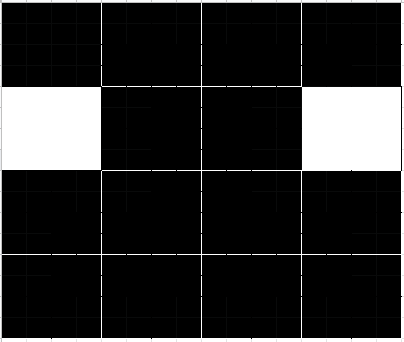
\includegraphics[width=.24\textwidth]{img/basico3.png}
    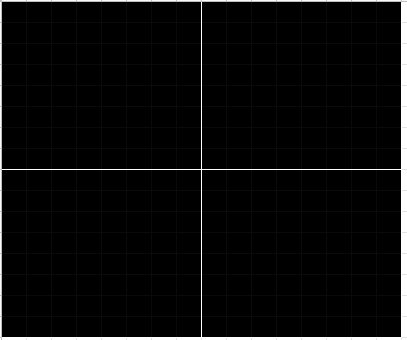
\includegraphics[width=.24\textwidth]{img/basico4.png}
    \caption{Simplificación algoritmo con r = 4 (Izquierda) y r = 8 (Derecha)}
    \label{fig:basico2}
\end{figure}



\section{Aplicación del método Box counting para el cálculo de la dimensión fractal de matrices binarias}

El algoritmo sobre el que se sustenta este proyecto tiene 3 características destacables:

\begin{itemize}
    \item \textbf{Método de escaneo}: Se trata de la manera que tenémos de recorrer la matriz, en el algoritmo utilizado para este proyecto se utiliza un método de escaneo de cuadrícula fija ( \textit{"fixed grid scans"} en inglés) \cite{unknown-author-no-dateF}. Esto quiere decir que a la hora de subdividir la estructura de datos en cajas, se hará de manera que para cada tamaño de caja seleccionado, un elemento de la matriz pertenecerá únicamente a una caja, sin que exista la posibilidad de que un elemento este en dos cajas para una misma subdivisión.
    \item \textbf{Criterio de validez}: Una vez tengamos la estructura de datos divididas en cajas del mismo tamaño, tenemos que establecer una regla para decidir sin contar la caja como válida o no. En este caso es necesario hacer una distinción:
    \begin{itemize}
        \item Sí  r = 1 , se cuenta el elemento como válido siempre que el elemento valga 1.
        \item Sí  r > 1 , se realiza una operación OR con todos los elementos de la caja. En caso de que el resultado de la operación sea 1 se contará la caja como válida. 
    \end{itemize}
    \item \textbf{Aumento del tamaño de la caja}: En cada iteración el tamaño de la caja aumenta siguiendo las potencias de 2 (1,2,4...) hasta llegar al tamaño de las dimensiones de la matriz. Se trabaja con matrices cuadradas con tamaños de fila o columna potencia de 2.
\end{itemize}


Como se adelanta en la última característica comentada, el cálculo de r no supone ninguna complicación, ya que conociendo el tamaño de la matriz cuadrada, simplemente consiste en crear una lista cuyos valores sean las potencias de 2 hasta el tamaño de la matriz.\\

Sin embargo, el cálculo de las cajas que cumplen el criterio de validez, es más complejo y requiere de un coste computacional bastante más elevado. En el Listado \ref{MatBox2D}, que corresponde a la implementación en Matlab de la que se parte como base para el proyecto \cite{unknown-author-2008}, se aprecia la aplicación del algoritmo para el cálculo de N (número de cajas válidas).\\

\begin{lstlisting}[language=Matlab,caption={Código Matlab del método Box counting para matrices bidimensionales. Las variables de entrada del código son la matriz c (matriz binaria que queremos analizar), la lista n (inicialmente vacía, contendrá el número de cajas válidas para cada tamaño de caja) y la variable p. que representa el número de iteraciones necesarias para cubrir la matriz entera, teniendo en cuenta que cada iteración aumenta el tamaño de la caja en una potencia de dos.},label=MatBox2D]
n(p+1) = sum(c(:));
for g=(p-1):-1:0
    $\Comment{//siz es el valor de r, es decir el tamaño de la caja}$
    siz = 2^(p-g);
    $\Comment{//siz2 es utilizada para localizar el resultado de }$
    $\Comment{//la operación OR del r de la anterior iteración. }$
    $\Comment{//Las casillas roja en las figuras de la sección 3.3 }$
    siz2 = round(siz/2);
    $\Comment{//Estos bucles son los encargados de realizar el cálculo del OR}$
    for i=1:siz:(width-siz+1)
        for j=1:siz:(width-siz+1)
            c(i,j) = ( c(i,j) || c(i+siz2,j) || ...
                                c(i,j+siz2) || c(i+siz2,j+siz2) );
        end
    end
    $\Comment{//Se acumula el número de 1 (se calcula el N para el r dado)}$
    n(g+1) = sum(sum(c(1:siz:(width-siz+1),1:siz:(width-siz+1))));
end
\end{lstlisting}

\section{Orden del algoritmo}
\label{Orden}
Para realizar un estudio del orden del algoritmo del Listado \ref{MatBox2D}, debemos diferenciar entre los bucles internos y el bucle  externo.\\

Los bucles internos, en el peor de los casos, tienen que recorrer la estructura de datos al completo (en dos ocasiones, líneas 10-15 y línea 17 en Listado \ref{MatBox2D}). Por tanto, la expresión \ref{eficiencia_interna} (donde el 2 representa las dos operaciones elementales previas, el cálculo de la variable siz y siz2) caracteriza el tiempo de ejecución del interior del bucle externo, es decir, el contenido de las líneas 3 - 17 . Como la notación O trata de acotar superiormente, podemos concluir que dicha parte del algoritmo tiene un orden de O($n^2$).\\

\begin{equation}
    \label{eficiencia_interna}
    n^2 + n^2 + 2 = 0
\end{equation}

Por otro lado, el bucle externo realiza un total de p iteraciones, siendo p el $log_2(n)$. Por tanto, la expresión \ref{eficiencia} caracteriza el tiempo de ejecución del código del Listado \ref{MatBox2D}, siendo acotada superiormente por $log_2(n)*n^2$, por lo que podemos decir que el código es de orden O( $log_2(n)*n^2$). 

\begin{equation}
    \label{eficiencia}
    log_2(n)*(n^2 + n^2 + 2) = 0
\end{equation}

Se recuerda que en este proyecto no se ha trabajado únicamente con matrices bidimensionales, si no que también se ha trabajado con matrices tridimensionales y cuatridimensionales. Conforme aumenta la complejidad de la estructura de datos, aumenta la complejidad para recorrerla, siendo el algoritmo de orden O($log_2(n)*n^3$) para matrices con tres dimensiones y O($log_2(n)*n^4$) para matrices con cuatro dimensiones.
\section{Ejemplo para una matriz bidimensional}
Con el objetivo de clarificar el funcionamiento del algoritmo se dejan las Figuras \ref{fig:alg1}, \ref{fig:alg2} y \ref{fig:alg3}, con la representación del funcionamiento del algoritmo para una matriz bidimensional de 16x16.

\begin{figure}[H]
    \centering
    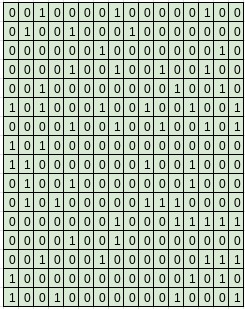
\includegraphics[width=.24\textwidth]{img/ejemploAlgoritmo1.jpeg}
    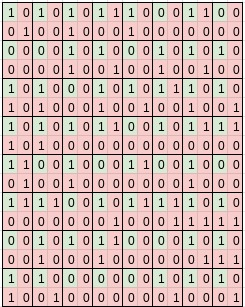
\includegraphics[width=.24\textwidth]{img/ejemploAlgoritmo2.jpeg}
    \caption{Iteraciones con r = 1 (Izquierda) y r = 2 (Derecha)}
    \label{fig:alg1}
\end{figure}

\begin{figure}[H]
    \centering
    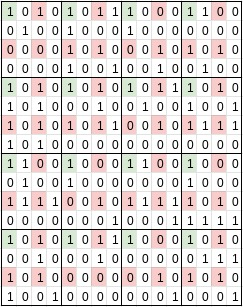
\includegraphics[width=.24\textwidth]{img/ejemploAlgoritmo3.jpeg}
    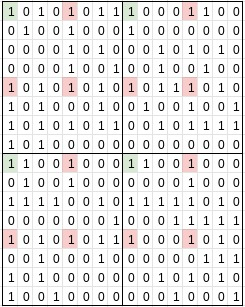
\includegraphics[width=.24\textwidth]{img/ejemploAlgoritmo4.jpeg}
    \caption{Iteraciones con r = 4 (Izquierda) y r = 8 (Derecha)}
    \label{fig:alg2}
\end{figure}

\begin{figure}[H]
    \centering
    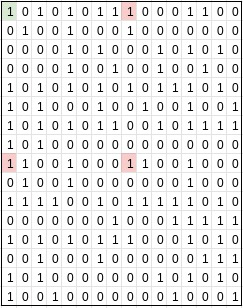
\includegraphics[width=.24\textwidth]{img/ejemploAlgoritmo5.jpeg}
    \caption{Iteracion con r = 16}
    \label{fig:alg3}
\end{figure}


Las casillas señaladas con el color verde corresponden a las casillas que son contadas a la hora de calcular el N (línea 16 en Listado \ref{MatBox2D}). Para el cálculo del valor de las casillas de color verde, se hace una operación OR con los valores calculados en la iteración anterior, es decir la casilla verde y las tres casillas señaladas de color rojo en las Figuras \ref{fig:alg1}, \ref{fig:alg2} y \ref{fig:alg3} (ver líneas 9-15 en Listado \ref{MatBox2D}).